% Usage: knitr slide

\chapter{Comparing Two Proportions} \ros{10.1-10.3, 10.5}\katz{5.2}\bmovie{8}\ddisc{8}

\section{Overview}

\bi
 \item Compare dichotomous independent variable with a dichotomous outcome
  \bi
  \item Independent variables: Exposed/Not, Treatment/Control, Knockout/Wild Type, etc.
  \item Outcome (dependent) variables: Diseased/Not or any Yes/No outcome 
  \ei
 \item Continuous outcomes often dichotomized for analysis (bad idea)
  \bi
  \item Consider $t$-tests (Chapter 5) or Non-parameteric methods (Chapter 7)
  \ei
\ei

\section{Normal-Approximation Test}
\bi
\item Two independent samples

%, sizes $n_{1}, n_{2}$
%\item Unknown population probabilities of event $p_{1}, p_{2}$
%\item Sample proportions for estimating $p_{1},p_{2}$: $\hat{p}_{1},
%  \hat{p}_{2}$
\begin{tabular}{lcc} 
 & \underline{Sample 1} & \underline{Sample 2} \\
Sample size & $n_1$ & $n_2$ \\
Population probability of event & $p_1$ & $p_2$ \\
Sample probability of event & $\hat{p}_1$ & $\hat{p}_2$ \\
\end{tabular}

\item Null Hypothesis, $H_{0}: p_{1}=p_{2}=p$
\item Estimating the variance
\bi 
 \item Variance of $\hat{p}_{i} = p_{i}(1-p_{i})/n_{i}$ for $i = 1, 2$
 \item Variance of $\left(\hat{p}_1 - \hat{p}_2\right)$ is the sum of the
  variances, which under $H_{0}$ is
   \beq
    p(1-p)[\frac{1}{n_{1}}+\frac{1}{n_{2}}]
   \eeq
 \item We estimate this variance by plugging $\hat{p}$ into $p$, where
 \beq
 \hat{p} = \frac{n_{1}\hat{p}_{1}+n_{2}\hat{p}_{2}}{n_{1}+n_{2}}
 \eeq
 is the pooled estimate of the probability under $H_{0}: p_1 = p_2 = p$
\ei
\item Test statistic which has approximately a normal distribution
  under $H_{0}$ if $n_{i}\hat{p}_{i}$ are each large enough:
\beq
z = \frac{\hat{p}_{1} -
  \hat{p}_{2}}{\sqrt{\hat{p}(1-\hat{p})[\frac{1}{n_{1}}+\frac{1}{n_{2}}]}}
\eeq
\item To test $H_{0}$ we see how likely it is to obtain a $z$ value as
  far or farther out in the tails of the normal distribution than $z$
  is
\item We don't recommend using the continuity correction
\item Example:  \\
Test whether the population of women whose age at first birth $\leq
29$ has the same probability of breast cancer as women whose age at
first birth was $\geq 30$.  This dichotomization is highly arbitrary
and we should really be testing for an association between age and
cancer incidence, treating age as a continuous variable.
\item Case-control study (independent and dependent variables
  interchanged); $p_{1}=$ probability of age at first birth $\geq 30$,
  etc.

\begin{tabular}{lcc} 
 & \underline{with Cancer} & \underline{without Cancer} \\
Total \# of subjects & $3220 (n_1)$ & $10245 (n_2)$ \\
\# age $\geq 30$ & $683$ & $1498$ \\ \\
Sample probabilities & $0.212 (\hat{p}_1$) & $0.146 (\hat{p}_2$) \\ \\
Pooled probability &\multicolumn{2}{c}{$\frac{683 + 1498}{3220 + 10245} = 0.162$} \\
\end{tabular}


%\beqa
%n_{1}=3220, n_{2}=10245, \\ 
%\hat{p}_{1}=\frac{683}{3220}=0.212, \\
%\hat{p}_{2}=\frac{1498}{10245} = 0.146 \\
%\hat{p}=\frac{683+1498}{3220+10245} = 0.162 \\
\item Estimate the variance
  \bi
  \item $\mathrm{variance}(\hat{p}_{1}-\hat{p}_{2}) = \hat{p}(1-\hat{p})\times \left[\frac{1}{n_{1}}+\frac{1}{n_{2}}\right] = 5.54 \times 10^{-5}$ \\
  \item $SE = \sqrt{\mathrm{variance}} = 0.00744$ \\
  \ei
\item Test statistic
  \bi 
  \item $z = \frac{0.212-0.146}{0.00744} = 8.85$
  \ei
\item 2-tailed $P$-value is $ < 10^{-4}$
\begin{Schunk}
\begin{Sinput}
n1 <- 3220;     n2 <- 10245
p1 <- 683 / n1; p2 <- 1498 / n2
pp <- (n1 * p1 + n2 * p2) / (n1 + n2)
se <- sqrt(pp * (1 - pp) * (1 / n1 + 1 / n2))
z  <- (p1 - p2) / se
pval <- 2 * (1 - pnorm(abs(z)))
round(c(p1=p1, p2=p2, pooled=pp, se=se, z=z, pval=pval), 4)
\end{Sinput}
\begin{Soutput}
    p1     p2 pooled     se      z   pval 
0.2121 0.1462 0.1620 0.0074 8.8527 0.0000 
\end{Soutput}
\end{Schunk}
\item We do not use a $t$-distribution because there is no $\sigma$ to
  estimate (and hence no ``denominator d.f.'' to subtract)
\ei

\section{$\chi^2$ Test}
\bi
\item If $z$ has a normal distribution, $z^2$ has a $\chi^2$
  distribution with 1 d.f. (are testing a single difference against zero)
\item The data we just tested can be shown as a $2\times 2$
  contingency table

\begin{tabular}{l|c|c|c} 
\multicolumn{1}{l}{} & \multicolumn{1}{c}{Cancer +} & \multicolumn{1}{l}{Cancer -} \\ \cline{2-3}
Age $\leq 29$ & $2537 $ & $8747$ & $11284$ \\ \cline{2-3}
Age $\geq 30$ & $683$ & $1498$ &  $2181$ \\ \cline{2-3}
\multicolumn{1}{l}{} & \multicolumn{1}{c}{$3220$} & \multicolumn{1}{c}{$10245$} & \multicolumn{1}{c}{$13465$}
\end{tabular}


\item In general, the $\chi^2$ test statistic is given by
\beq
\sum_{ij} \frac{(\textrm{Obs}_{ij}-\textrm{Exp}_{ij})^2}{\textrm{Exp}_{ij}}
% \frac{(\textrm{Observed_{ij}} - \textrm{Expected_{ij}})^2}{\textrm{Expected_{ij}}}$
\eeq
\item $\textrm{Obs}_{ij}$ is the observed cell frequency for row $i$ column $j$
\item $\textrm{Exp}_{ij}$ is the expected cell frequency for row $i$ column $j$
  \bi
  \item Expected cell frequencies calculating assuming $H_0$ is true
  \item $\textrm{Exp}_{ij} = \frac{\textrm{row $i$ total} \times \textrm{column $j$ total}}{\textrm{grand total}}$
  \item e.g. $\textrm{Exp}_{11} = \frac{11284 \times 3220}{13465} = 2698.4$
  \ei

\item For $2 \times 2$ tables, if the observed cell frequencies are labeled
\begin{tabular}{|c|c|} \hline
$a$ & $b$ \\ \hline
$c$ & $d$ \\ \hline
\end{tabular}
the $\chi^{2}$ test statistic simplifies to
\beq
\frac{N[ad - bc]^{2}}{(a+c)(b+d)(a+b)(c+d)},
\eeq
where $N=a+b+c+d$.  Here we get $\chi^{2}_{1} = 78.37$
\item 78.37 is $z^2$ from above!
\begin{Schunk}
\begin{Sinput}
x <- matrix(c(2537, 8747, 683, 1498), nrow=2, byrow=TRUE)
x
\end{Sinput}
\begin{Soutput}
     [,1] [,2]
[1,] 2537 8747
[2,]  683 1498
\end{Soutput}
\begin{Sinput}
chisq.test(x, correct=FALSE)
\end{Sinput}
\begin{Soutput}

	Pearson's Chi-squared test

data:  x
X-squared = 78.37, df = 1, p-value < 2.2e-16
\end{Soutput}
\begin{Sinput}
# Also compute more accurate P-value based on 1M Monte-Carlo simulations
chisq.test(x, correct=FALSE, simulate.p.value=TRUE, B=1e6)
\end{Sinput}
\begin{Soutput}

	Pearson's Chi-squared test with simulated p-value (based on 1e+06
	replicates)

data:  x
X-squared = 78.37, df = NA, p-value = 1e-06
\end{Soutput}
\end{Schunk}
\item Don't need Yates' continuity correction
%  Eq.\ 10.5
\item Note that even though we are doing a 2-tailed
test we use only the right tail of the $\chi^{2}_{1}$ distribution;
that's because we have squared the difference when computing the
statistic, so the sign is lost.
\item This is the ordinary Pearson $\chi^2$ test
\ei

\section{Fisher's Exact Test}
\bi
\item Is a misnomer in the sense that it computes probabilities
  exactly, with no normal approximation, but only after changing what
  is being tested to condition on the number of events and non-events
\item Because frequencies are discrete and because of the
  conditioning, the test is conservative ($P$-values too large)
\item Is exact only in the sense that actual type I error probability will not \textbf{exceed} the nominal level
\item The ordinary Pearson $\chi^2$ works fine (even when
  an expected cell frequency is as low as 1.0, contrary to popular belief)
\item We don't use Yates' continuity correction because it was
  developed to make the normal approximation test yield $P$-values
  that are more similar to Fisher's test, i.e., to be more
  conservative
\item The attempt to obtain exact unconditional $P$-values for the simple $2\times 2$ contingency table has stumped frequentist statisticians for many decades~\cite{cho15elu}
\item By contrast, Bayesian posterior probabilities for the true unconditional quantity of interest are exact
 \bi
 \item Frequentist confidence limits and $P$-values are approximate because they use the sample space, and the sample space is discrete when the response variable is categorical
 \item Bayes does not consider the sample space, only the parameter space, which is almost always continuous
 \ei
\item See \href{https://stats.stackexchange.com/questions/14226}{stats.stackexchange.com/questions/14226} for discussion
\ei

\section{Sample Size and Power for Comparing Two Independent Samples}
\bi
\item Power $\uparrow$ as
 \bi
 \item $n_{1}, n_{2} \uparrow$
 \item $\frac{n_{2}}{n_{1}} \rightarrow 1.0$ (usually)
 \item $\Delta = |p_{1}-p_{2}| \uparrow$
 \item $\alpha \uparrow$
 \ei
\item There are approximate formulas such as the recommended methods in Altman based on transforming $\hat{p}$ to make it have a
  variance that is almost independent of $p$ \altman{45-50}
\item Example:  \\

Using current therapy, 0.5 of the population is free of infection at 24 hours.  Adding a new drug to the standard of care is expected to increase the percentage infection-free to 0.7.  If we randomly sample 100 subjects to receive standard care and 100 subjects to receive the new therapy, what is the probabilty that we will be able to detect a certain difference between the two therapies at the end of the study?

\beq
p_{1}=.5, p_{2}=.7, n_{1}=n_{2}=100
\eeq
results in a power of 0.83 when $\alpha=0.05$
\begin{Schunk}
\begin{Sinput}
require(Hmisc)
bpower(.5, .7, n1=100, n2=100)
\end{Sinput}
\begin{Soutput}
    Power 
0.8281098 
\end{Soutput}
\end{Schunk}
\item When computing sample size to achieve a given power, the sample
  size $\downarrow$ when
 \bi
 \item power $\downarrow$
 \item $\frac{n_{2}}{n_{1}} \rightarrow 1.0$
 \item $\Delta \uparrow$
 \item $\alpha \uparrow$
 \ei
\item Required sample size is a function of both $p_{1}$ and $p_{2}$
\item Example:

How many subjects are needed to detect a 0.8 fold decrease in the probability of colorectal cancer if the baseline probability of cancer is $0.0015$?  Use a power of 0.8 and a type-I error probability of 0.05.

\beqa
p_{1}=0.0015, p_{2}=0.8\times p_{1}=0.0012, \alpha=0.05, \beta=0.2 \\
n_{1}=n_{2}=235,147
\eeqa
(Rosner estimated 234,881)
\ei
\begin{Schunk}
\begin{Sinput}
bsamsize(.0015, 0.8 * .0015, alpha=0.05, power=0.8)
\end{Sinput}
\begin{Soutput}
      n1       n2 
235147.3 235147.3 
\end{Soutput}
\end{Schunk}

Formulas for power and sample size may be seen as \R\ code found at\\
\href{https://github.com/harrelfe/Hmisc/blob/master/R/bpower.s}{github.com/harrelfe/Hmisc/blob/master/R/bpower.s}.

\section{Confidence Interval}
An approximate $1-\alpha$ 2-sided CL is given by
\beq
\hat{p}_{1}-\hat{p}_{2} \pm z_{1-\alpha/2} \times\sqrt{\frac{\hat{p}_{1}(1-\hat{p}_{1})}{n_{1}}+\frac{\hat{p}_{2}(1-\hat{p}_{2})}{n_{2}}}
\eeq
where $z_{1-\alpha/2}$ is the critical value from the normal
distribution (1.96 when $\alpha=0.05$).

The CL for the number of patients needed to be treated to save one
event may simply be obtained by taking the reciprocal of the two
confidence limits.\footnote{If a negative risk reduction is included
  in the confidence interval, set the NNT to $\infty$ for that limit
  instead of quoting a negative NNT.  There is more to this; see \href{http://bit.ly/datamethods-nnt}{bit.ly/datamethods-nnt}.}

\section{Sample Size for a Given Precision}

\bi
 \item Goal: Plan a study so that the margin of error is sufficiently small
 \item The margin of error ($\delta$) is defined to be half of the confidence interval width.  For two proportions,
  \beq
  \delta = z_{1-\alpha/2} \times\sqrt{\frac{\hat{p}_{1}(1-\hat{p}_{1})}{n_{1}}+\frac{\hat{p}_{2}(1-\hat{p}_{2})}{n_{2}}}
  \eeq
 \item Basing the sample size calculations on the margin of error can lead to a study that gives \textit{scientifically} relevant results even if the results are not \textit{statistically} significant.
  \item Example: Suppose that the infection risk in a population is $0.5$ and a reduction to $0.4$ is believed to be a large enough reduction that it would lead to a change in procedures.  A study of a new treatment is planned so that enough subjects will be enrolled for the margin of error is $0.05$.  Consider these two possible outcomes:
  \begin{enumerate}
  \item The new treatment is observed to decrease infections by $0.06$ ($0.95$ CI: $[0.11, 0.01]$).  The confidence interval does not contain $0$, so we have indirect evidence\footnote{To obtain direct evidence requires Bayesian posterior probabilities.} that the new treatment is effective at reducing infections.  $0.1$ is also within the confidence interval limits.
  \item The new treatment is observed to decrease infections by only $0.04$ ($0.95$ CI: $[0.09, -0.01]$).  The confidence interval now contains $0$, so we do not have enough evidence to reject the supposition that there is no effect of the treatment on reducing infections if we are bound to an arbitrary $\alpha=0.05$. However, the confidence interval also does not contain $0.10$, so we are able to indirectly rule out a \textit{scientifically} relevant decrease in infections.
  \end{enumerate}


 \item For fixed $n_{1} = n_2 = n$, confidence intervals for proportions have the maximum width, when $p_{1} = p_{2} =  0.5$.  This can be shown by:
  \bi
  \item Recall that the variance formula for the difference in two proportions when calculating a confidence interval is 
   \beq
   \frac{p_{1}(1-p_{1})}{n_{1}}+\frac{p_{2}(1-p_{2})}{n_{2}}
    \eeq
  \item When $p_{1} = p_{2} =  p$ and $n_{1} = n_2 = n$, the variance formula simplifies to 
    \beq
     \frac{p(1 - p)}{n}+\frac{p (1- p)}{n} = 2\frac{p(1 - p)}{n}
    \eeq
   \item Then, for any fixed value of $n$ ($e.g. n = 1$ or $10$), $2\frac{p(1 - p)}{n}$ is largest when $p = 0.5$.  With $p= 0.5$, the variance formula further simplifies to
    \beq
     2\frac{.25}{n} = \frac{1}{2n}
    \eeq
  \ei
 \item Using $\alpha = 0.05$ ($z_{1-\alpha/2} = 1.96$), the worst-case margin of error will be
    \beq
     \delta = 1.96 \sqrt{\frac{1}{2n}}
    \eeq
 \item By solving for $n$, we can rearrange this formula to be
    \beq
     n = \frac{1.92}{\delta^2}
    \eeq
 \item This formula then gives the number of subjects needed in each group $n$ to obtain a given margin of error $\delta$.  For a margin of error of $0.05$ ($\delta = 0.05$), $n = \frac{1.92}{0.05^2} = 768$ subjects in each group.
\begin{Schunk}
\begin{Sinput}
diff <- .05
qnorm(.975)^2 / 2 / (diff ^ 2)
\end{Sinput}
\begin{Soutput}
[1] 768.2918
\end{Soutput}
\end{Schunk}
\ei

%In the case $n_{1}=n_{2}=n, \alpha=0.05$, the confidence interval has maximum width with $p_{1}$ and $p_{2}$ are near 0.5.  As a worse case the margin of error is then $1.96/\sqrt{2n}$.  The $n$ required to achieve a margin of error of $\delta$ at the 0.95 confidence level is $1.92/\delta^{2}$.  For example, to approximate the difference in the incidence probability of stroke between males and females to at worst $\pm 0.05$ at the 0.95 level would require 768 patients in each group.

\section{Relative Effect Measures}\alabel{sec:prop-rem}
\bi
\item We have been dealing with risk differences which are measures of
  absolute effect
\item Measures of relative effect include risk ratios and odds ratios
\item Risk ratios are easier to interpret but only are useful over a
  limited range of prognosis (i.e., a risk factor that doubles your
  risk of lung cancer cannot apply to a subject having a risk above
  0.5 without the risk factor)
\item Odds ratios can apply to any subject
\item In large clinical trials treatment effects on lowering
  probability of an event are often constant on the odds ratio scale
\item OR = Odds ratio =
  $\frac{\frac{p_{1}}{1-p_{1}}}{\frac{p_{2}}{1-p_{2}}}$
\item Testing $H_{0}$: OR=1 is equivalent to testing
  $H_{0}:p_{1}=p_{2}$
\item There are formulas for computing confidence intervals for odds
  ratios
\item Odds ratios are most variable when one or both of the
  probabilities are near 0 or 1
\item We compute CLs for ORs by anti-logging CLs for the log OR
\item In the case where $p_{1}=p_{2}=0.05$ and $n_{1}=n_{2}=n$, the
  standard error of the log odds ratio is approximately
  $\sqrt{\frac{42.1}{n}}$
\item The common sample size $n$ needed to estimate the true OR to
  within a factor of 1.5 is 984 with $p$s in this range
\item To show the multiplicative margins of error\footnote{Value by
    which to multiply the observed odds ratio to obtain the upper 0.95
    confidence limit or to divide the observed odds ratio to obtain
    the lower 0.95 limit} for a range of sample sizes and values of
  $p$.  For each scenario, the margin of error assumes that both
  unknown probability estimates equal $p$.
\ei
\begin{Schunk}
\begin{Sinput}
require(ggplot2)
d <- expand.grid(n=c(seq(10, 1000, by=10), seq(1100, 50000, by=100)),
                 p=c(.02, .05, .075, .1, .15, .2, .25, .3, .4, .5))
d$selor <- with(d, sqrt(2 / (p * (1 - p) * n)))
d$mmoe  <- with(d, exp(qnorm(0.975) * selor))
mb <- c(1, 1.25, 1.5, 2, 2.5, 3, 4, 5, 10, 20, 30, 40, 50, 100, 400)
ggplot(aes(x=n, y=mmoe, color=factor(p)), data=d) +   # Fig. (*\ref{fig:prop-mmeor}*)
  geom_line() +
  scale_x_log10(breaks=c(10,20,30,50,100,200,500,1000,2000,5000,10000,
                  20000,50000)) +
  scale_y_log10(breaks=mb, labels=as.character(mb)) +
  xlab(expression(n)) + ylab('Multiplicative Margin of Error for OR') +
  guides(color=guide_legend(title=expression(p)))
\end{Sinput}
\begin{figure}[htbp]

\centerline{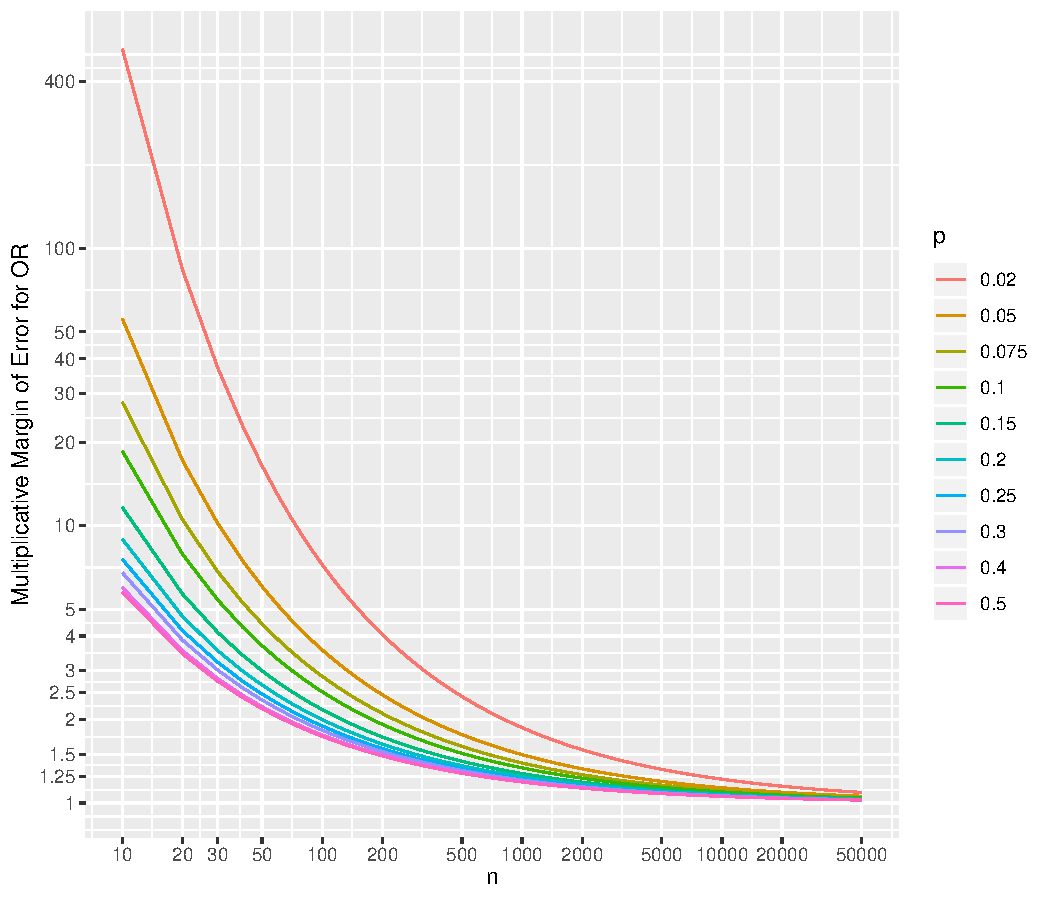
\includegraphics[width=\maxwidth]{prop-mmeor-1} }

\caption[Multiplicative margin of error for odds ratios]{Multiplicative margin of error related to 0.95 confidence limits of an odds ratio, for varying $n$ and $p$ (different curves), assuming the unknown true probability in each group is no lower than $p$}\label{fig:prop-mmeor}
\end{figure}
\end{Schunk}


\section{Comprehensive example}

\subsection{Study Description}
\bi
  \item Consider patients who will undergo coronary artery bypass graft surgery (CABG)
  \item Mortality risk associated with open heart surgery
  \item Study question: Do emergency cases have a surgical mortality that is different from that of non-emergency cases?
  \item Population probabilities
  \bi
    \item $p_1$: Probability of death in patients with emergency priority
    \item $p_2$: Probability of death in patients with non-emergency priority
  \ei
  \item Statistical hypotheses
  \bi
  \item $H_0: p_1 = p_2$ (or $\textrm{OR} = 1$)
  \item $H_1: p_1 \neq p_2$ (or $\textrm{OR} \neq 1$)
  \ei
\ei

\subsection{Power and Sample Size}

\bi
  \item Prior research shows that just over $0.1$ of surgeries end in death
  \item Researchers want to be able to detect a 3 fold increase in risk
  \item For every 1 emergency priority, expect to see 10 non-emergency
  \item $p_1 = 0.3$, $p_2 = 0.1$, $\alpha = 0.05$, and $\textrm{power} = 0.90$
  \item Calculate sample sizes using the PS software for these values and other combinations of $p_1$ and $p_2$
\ei

\begin{table}[!hbp]
 \begin{center}
 \begin{tabular}{lcccc} \hline\hline
$(p_1, p_2)$ &\boldmath$(0.3, 0.1)$&$(0.4, 0.2)$&$(0.03, 0.01)$&$(0.7, 0.9)$ \\ 
$n_1$  &\boldmath$40$&$56$&$589$&$40$ \\ 
$n_2$  &\boldmath$400$&$560$&$5890$&$400$ \\ \hline \hline
\end{tabular}
\end{center}
\end{table}
Check PS calculations against the \R\ \Co{Hmisc} package's
\Co{bsamsize} function.
\begin{Schunk}
\begin{Sinput}
round(bsamsize(.3, .1, fraction=1/11, power=.9))
\end{Sinput}
\begin{Soutput}
 n1  n2 
 40 399 
\end{Soutput}
\begin{Sinput}
round(bsamsize(.4, .2, fraction=1/11, power=.9))
\end{Sinput}
\begin{Soutput}
 n1  n2 
 56 561 
\end{Soutput}
\begin{Sinput}
round(bsamsize(.7, .9, fraction=1/11, power=.9))
\end{Sinput}
\begin{Soutput}
 n1  n2 
 40 399 
\end{Soutput}
\end{Schunk}

\subsection{Collected Data}

In-hospital mortality figures for emergency surgery and other surgery

\begin{table}[!hbp]
 \begin{center}
 \begin{tabular}{l|cc}
 & \multicolumn{2}{|c}{Discharge Status} \\
Surgical Priority& Dead& Alive \\ \hline
Emergency&$6$&$ 19$\\
Other&$11$&$100$\\
\end{tabular}
\end{center}
\end{table}

\bi
\item $\hat{p}_1 = \frac{6}{25} = 0.24$
\item $\hat{p}_2 = \frac{11}{111} = 0.10$
\ei

\subsection{Statistical Test}
\begin{Schunk}
\begin{Sinput}
n1 <- 25;     n2 <- 111
p1 <- 6 / n1; p2 <- 11 / n2
or <- p1 / (1 - p1) / (p2 / (1 - p2))
or
\end{Sinput}
\begin{Soutput}
[1] 2.870813
\end{Soutput}
\begin{Sinput}
# Standard error of log odds ratio:
selor <- sqrt(1 / (n1 * p1 * (1 - p1)) + 1 / (n2 * p2 * (1 - p2)))
# Get 0.95 confidence limits
cls <- exp(log(or) + c(-1, 1) * qnorm(0.975) * selor)
cls
\end{Sinput}
\begin{Soutput}
[1] 0.946971 8.703085
\end{Soutput}
\begin{Sinput}
tcls <- paste0(round(or, 2), ' (0.95 CI: [', round(cls[1], 2),
               ', ', round(cls[2], 2), '])')
# Multiplying a constant by the vector -1, 1 does +/-
x <- matrix(c(6, 19, 11, 100), nrow=2, byrow=TRUE)
x
\end{Sinput}
\begin{Soutput}
     [,1] [,2]
[1,]    6   19
[2,]   11  100
\end{Soutput}
\begin{Sinput}
chisq.test(x, correct=FALSE)
\end{Sinput}
\begin{Soutput}

	Pearson's Chi-squared test

data:  x
X-squared = 3.7037, df = 1, p-value = 0.05429
\end{Soutput}
\end{Schunk}
% Ignore the warning about the $\chi^2$ approximation.
\bi
\item Interpretation
 \bi
 \item Compare odds of death in the emergency group
   $\left(\frac{\hat{p}_1}{1-\hat{p}_1}\right)$ to odds of death in
   non-emergency group  $\left(\frac{\hat{p}_2}{1-\hat{p}_2}\right)$ 
 \item Emergency cases have 2.87 (0.95 CI: [0.95, 8.7]) fold
   increased odds of death during surgery compared to
   non-emergency cases. 
 \ei
\ei

\subsubsection{Fisher's Exact Test}

Observed marginal totals from emergency surgery dataset \\
\begin{tabular}{l|c|c|c} 
\multicolumn{1}{l}{} & \multicolumn{1}{c}{Dead} & \multicolumn{1}{l}{Alive} \\ \cline{2-3}
Emergency & $a$ & $b$ & $25$ \\ \cline{2-3}
Other & $c$ & $d$ &  $111$ \\ \cline{2-3}
\multicolumn{1}{l}{} & \multicolumn{1}{c}{$17$} & \multicolumn{1}{c}{$119$} & \multicolumn{1}{c}{$136$}
\end{tabular}

\bi
\item With fixed marginal totals, there are 18 possible tables ($a = 0, 1, \ldots 17$)
\item Can calculated probability of each of these tables
\bi
\item $p$-value: Probability of observing data as extreme or more extreme than we collected in this experiment
\ei
\item Exact test: $p$-value can be calculated ``exactly'' (not using the $\chi^2$ distribution to approximate the $p$-value)
\\
\begin{Schunk}
\begin{Sinput}
fisher.test(x)
\end{Sinput}
\begin{Soutput}

	Fisher's Exact Test for Count Data

data:  x
p-value = 0.08706
alternative hypothesis: true odds ratio is not equal to 1
95 percent confidence interval:
 0.7674155 9.6831351
sample estimates:
odds ratio 
  2.843047 
\end{Soutput}
\end{Schunk}
Note that the odds ratio from Fisher's test is a conditional maximum
likelihood estimate, which differs from the unconditional maximum
likelihood estimate we obtained earlier.
\item Fisher's test more conservative than Pearson's $\chi^2$ test
  (larger $P$-value) 
\ei

\section{Logistic Regression for Comparing Proportions}\bmovie{9}\ddisc{9}
\bi
\item When comparing $\geq 2$ groups on the probability that a categorical outcome variable will have a certain value observed (e.g., $P(Y=1)$), one can use the Pearson $\chi^2$ test for a contengency table (or the less powerful Fisher's ``exact'' test)
\item Such analyses can also be done with a variety of regression models
\item It is necessary to use a regression model when one desires to analyze more than the grouping variable, e.g.
  \bi
  \item analyze effects of two grouping variables
  \item adjust for covariates
  \ei
\item For full generality, the regression model needs to have no restrictions on the regression coefficients
  \bi
  \item Probabilities are restricted to be in the interval $[0,1]$ so an additive risk model cannot fit over a broad risk range
  \item Odds ($\frac{p}{1-p}$) are restricted to be in $[0, \infty]$
  \item Log odds have no restrictions since they can be in $[-\infty, \infty]$
  \ei
\item So log odds is a good basis for regression analysis of categorical $Y$
 \bi
 \item default assumption of additivity of effects needs no restrictions
 \item will still translate to probabilities in $[0,1]$
 \ei
\item The binary logistic regression model is a model to estimate the probability of an event as a flexible function of covariates
\item Let the outcome variable $Y$ have the values $Y=0$ (non-event) or $Y=1$ (event)
\begin{equation}
  \textrm{Prob}(Y = 1 | X) = \frac{1}{1 + \exp(-(\beta_0 + \beta_1 x_1 + \beta_2 x_2 + \beta_3 x_3 + \ldots))}
\end{equation}
\item The sum inside the inner () is called the linear predictor (LP)
\item The binary logistic model relates LP (with no restrictions) to the event probability as so:
\begin{Schunk}
\begin{Sinput}
lp <- seq(-5, 5, length=150)
plot(lp, plogis(lp), xlab='Linear Predictor', ylab='P(Y=1)', type='l')
\end{Sinput}


\centerline{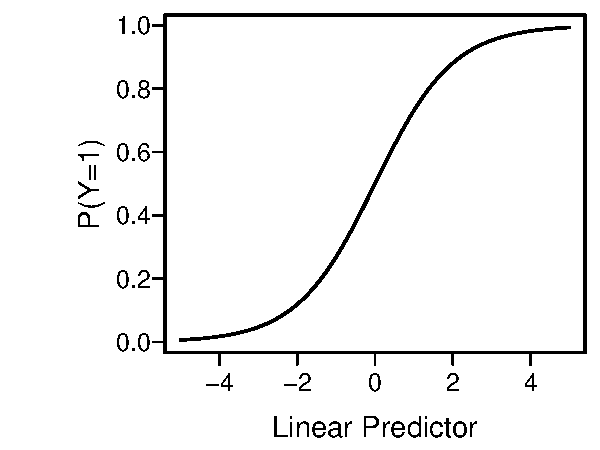
\includegraphics[width=\maxwidth]{prop-lrmshape-1} }

\end{Schunk}
\item Notes about LP:
 \bi 
 \item for a given problem the range may be much narrower than $[-4,4]$
 \item when any predictor $X_j$ with a non-zero $\beta_j$ is categorical, LP cannot take on all possible values within its range, so the above plot will have gaps
 \ei
\item As a special case the model can estimate and compare two probabilities as done above, through an odds ratio
\item Logistic regression seems like an overkill here, but it sets the stage for more complex frequentist analysis as well as Bayesian analysis
\item For our case the model is as follows
\item Consider groups A and B, A = reference group\\
  $[x]$ denotes 1 if $x$ is true, 0 if $x$ is false\\
  Define the expit function as the inverse of the logit function, or expit$(x) = \frac{1}{1 + \exp(-x)}$
\beqa
P(Y = 1 | \textrm{group}) &=& \frac{1}{1 + \exp(-(\beta_0 + \beta_1 [\textrm{group } B]))} \\
 &=& \textrm{expit}(\beta_0 + \beta_1 [\textrm{group } B])\\
P(Y = 1 | \textrm{group A}) &=& \textrm{expit}(\beta_0)\\
P(Y = 1 | \textrm{group B}) &=& \textrm{expit}(\beta_0 + \beta_1)
\eeqa
$\beta_0 =$ log odds of probability of event in group A $= \log(\frac{p_1}{1 - p_1}) = \textrm{logit}(p_1)$\\
$\beta_1 =$ increase in log odds in going from group A to group B = \\ $\log(\frac{p_2}{1 - p_2}) - \log(\frac{p_1}{1 - p_1}) = \textrm{logit}(p_2) - \textrm{logit}(p_1)$\\
$\exp(\beta_1) =$ group B : group A odds ratio $= \frac{\frac{p_2}{1 - p_2}}{\frac{p_1}{1 - p_1}}$ \\
expit$(\beta_0) = p_1$ \\
expit$(\beta_0 + \beta_1) = p_2$
\item Once the $\beta$s are estimated, one quickly gets the B:A odds ratio and $\hat{p}_1$ and $\hat{p}_2$
\item This model is \textbf{saturated}
 \bi
 \item has the maximum number of parameters needed to fully describe the situation (here, 2 since 2 groups)
 \item saturated models \textbf{must} fit the data if the distributional and independence assumptions are met 
 \item logistic model has no distributional assumption
 \ei 
\item Logistic regression is more general and flexible than the specialized tests for proportions
 \bi
 \item allows testing association on continuous characteristics
 \item easily extends to more than two groups
 \item allows adjustment for covariates
 \ei
\item Examples:\\
  \bi
  \item assess effects of subjects' sex and country (Canada vs.\ US) on $P(Y=1)$ denoted by $p$\\
  logit $p$ = constant + logit male effect + logit Canada effect
  \item same but allow for interaction\\
  logit $p$ = constant + logit male effect + logit Canada effect + special effect of being male if Canadian
  \item latter model is saturated with 3 d.f.\ so fits as well as a model with 4 proportions
    \bi
    \item unlike the overall Pearson $\chi^2$ test, allows testing interaction and
    \item separate effects of sex and country (e.g., 2 d.f.\ chunk test for whether there is a sex difference for either country, allowing for the sex effect to differ by country)
    \ei
  \ei
\ei

\subsection{Test Statistics}
For frequentist logistic models there are 3 types of $\chi^2$ test statistics for testing the same hypothesis:
  \bi
  \item likelihood ratio (LR) test (usually the most accurate) and is scale invariant\footnote{The LR test statistic is the same whether testing for an absolute risk difference of 0.0, or for an odds or risk ratio of 1.0.}
   \bi
   \item Can obtain the likelihood ratio $\chi^2$ statistic from either the logistic model or from a logarithmic equation in the two proportions and sample sizes
   \ei
  \item Score test (identical to Pearson test for overall model if model is saturated)
  \item Wald test (square of $\frac{\hat{\beta}}{\textrm{s.e.}}$ in the one parameter case; misbehaves for extremely large effects)
  \item Wald test is the easiest to compute but $P$-values and confidence intervals from it are not as accurate.  The score test is the way to exactly reproduce the Pearson $\chi^2$ statistic from the logistic model.
  \item As with $t$-test vs.\ a linear model, the special case tests are not needed once you use the logistic model framework
  \item Three usages of any of these test statistics:
    \bi
    \item individual test, e.g. sex effect in sex-country model without interaction
    \item chunk test, e.g. sex + sex $\times$ country interaction 2 d.f.\ test\\tests overall sex effect
    \item global test of no association, e.g. 3 d.f.\ test for whether sex or country is associated with $Y$
    \ei
  \ei
 
\subsection{Frequentist Analysis Example}
 \bi
 \item Consider again our emergency surgery example
 \item String the observations out to get one row = one patient, binary $Y$
 \ei

\begin{Schunk}
\begin{Sinput}
require(rms)
options(prType='latex')
priority <- factor(c(rep('emergency', 25), rep('other', 111)), c('other', 'emergency'))
death <- c(rep(0, 19), rep(1, 6), rep(0, 100), rep(1, 11))
table(priority, death)
\end{Sinput}
\begin{Soutput}
           death
priority      0   1
  other     100  11
  emergency  19   6
\end{Soutput}
\end{Schunk}
\begin{Sinput}
d  <- data.frame(priority, death)
dd <- datadist(d); options(datadist='dd')
# rms package needs covariate summaries computed by datadist
f <- lrm(death ~ priority)
f
\end{Sinput}

 \centerline{\textbf{Logistic Regression Model}}
 
 \begin{verbatim}
 lrm(formula = death ~ priority)
 \end{verbatim}
 
 {\fontfamily{phv}\selectfont \begin{center}\begin{tabular}{|c|c|c|c|}\hline
&Model Likelihood&Discrimination&Rank Discrim.\\
&Ratio Test&Indexes&Indexes\\\hline
Obs~\hfill 136&LR $\chi^{2}$~\hfill 3.20&$R^{2}$~\hfill 0.044&$C$~\hfill 0.597\\
~~0~\hfill 119&d.f.~\hfill 1&$g$~\hfill 0.319&$D_{xy}$~\hfill 0.193\\
~~1~\hfill 17&Pr$(>\chi^{2})$~\hfill 0.0737&$g_{r}$~\hfill 1.375&$\gamma$~\hfill 0.483\\
$\max|\frac{\partial\log L}{\partial \beta}|$~\hfill $4\!\times\!10^{-9}$&&$g_{p}$~\hfill 0.043&$\tau_{a}$~\hfill 0.043\\
&&Brier~\hfill 0.106&\\
\hline
\end{tabular}
\end{center}}
 
 %latex.default(U, file = "", first.hline.double = FALSE, table = FALSE,     longtable = TRUE, lines.page = lines.page, col.just = rep("r",         ncol(U)), rowlabel = "", already.math.col.names = TRUE,     append = TRUE)%
 \setlongtables\begin{longtable}{lrrrr}\hline
 \multicolumn{1}{l}{}&\multicolumn{1}{c}{$\hat{\beta}$}&\multicolumn{1}{c}{S.E.}&\multicolumn{1}{c}{Wald $Z$}&\multicolumn{1}{c}{Pr$(>|Z|)$}\tabularnewline
 \hline
 \endhead
 \hline
 \endfoot
 Intercept&~-2.2073~&~0.3177~&-6.95&\textless 0.0001\tabularnewline
 priority=emergency&~ 1.0546~&~0.5659~& 1.86&0.0624\tabularnewline
 \hline
 \end{longtable}
 \addtocounter{table}{-1}

\bi 
\item Compare the LR $\chi^2$ of 3.2 with the earlier Pearson $\chi^2$ of 3.70
\item The likelihood ratio (LR) $\chi^2$ test statistic and its $P$-value are usually a little more accurate than the other association tests
 \bi
 \item but $\chi^2$ distribution is still only an approximation to the true sampling distribution
 \ei
\item See that we can recover the simple proportions from the fitted logistic model:\\
$\hat{p}_1 = \frac{11}{111} = 0.099 = \textrm{expit}(-2.2073)$\\
$\hat{p}_2 = \frac{6}{25} = 0.24 = \textrm{expit}(-2.2073 + 1.0546)$
\ei 

\begin{Sinput}
summary(f)
\end{Sinput}
%latex.default(cstats, caption = if (table.env) caption else NULL,     title = title, rowlabel = "", col.just = rep("r", 7), table.env = table.env,     ...)%
\begin{center}
\begin{tabular}{lrrrrrrr}
\hline\hline
\multicolumn{1}{l}{}&\multicolumn{1}{c}{Low}&\multicolumn{1}{c}{High}&\multicolumn{1}{c}{$\Delta$}&\multicolumn{1}{c}{Effect}&\multicolumn{1}{c}{S.E.}&\multicolumn{1}{c}{Lower 0.95}&\multicolumn{1}{c}{Upper 0.95}\tabularnewline
\hline
priority --- emergency:other&1&2&&1.0546&0.56587&-0.054487&2.1637\tabularnewline
~~{\it Odds Ratio}&1&2&&2.8708&& 0.946970&8.7031\tabularnewline
\hline
\end{tabular}\end{center}


\bi
\item The point estimate and CLs for the odds ratio is the same as what we obtained earlier.
\ei

Add a random binary variable to the logistic model---one that is correlated with the surgical priorty---to see the effect on the estimate of the priority effect

\begin{Schunk}
\begin{Sinput}
set.seed(10)
randomUniform <- runif(length(priority))
random <- ifelse(priority == 'emergency', randomUniform < 1/3,
                                          randomUniform > 1/3) * 1
d$random <- random
table(priority, random)
\end{Sinput}
\begin{Soutput}
           random
priority     0  1
  other     39 72
  emergency 17  8
\end{Soutput}
\end{Schunk}
\begin{Sinput}
lrm(death ~ priority + random)
\end{Sinput}

 \centerline{\textbf{Logistic Regression Model}}
 
 \begin{verbatim}
 lrm(formula = death ~ priority + random)
 \end{verbatim}
 
 {\fontfamily{phv}\selectfont \begin{center}\begin{tabular}{|c|c|c|c|}\hline
&Model Likelihood&Discrimination&Rank Discrim.\\
&Ratio Test&Indexes&Indexes\\\hline
Obs~\hfill 136&LR $\chi^{2}$~\hfill 6.03&$R^{2}$~\hfill 0.082&$C$~\hfill 0.659\\
~~0~\hfill 119&d.f.~\hfill 2&$g$~\hfill 0.638&$D_{xy}$~\hfill 0.319\\
~~1~\hfill 17&Pr$(>\chi^{2})$~\hfill 0.0489&$g_{r}$~\hfill 1.892&$\gamma$~\hfill 0.464\\
$\max|\frac{\partial\log L}{\partial \beta}|$~\hfill $1\!\times\!10^{-8}$&&$g_{p}$~\hfill 0.073&$\tau_{a}$~\hfill 0.070\\
&&Brier~\hfill 0.103&\\
\hline
\end{tabular}
\end{center}}
 
 %latex.default(U, file = "", first.hline.double = FALSE, table = FALSE,     longtable = TRUE, lines.page = lines.page, col.just = rep("r",         ncol(U)), rowlabel = "", already.math.col.names = TRUE,     append = TRUE)%
 \setlongtables\begin{longtable}{lrrrr}\hline
 \multicolumn{1}{l}{}&\multicolumn{1}{c}{$\hat{\beta}$}&\multicolumn{1}{c}{S.E.}&\multicolumn{1}{c}{Wald $Z$}&\multicolumn{1}{c}{Pr$(>|Z|)$}\tabularnewline
 \hline
 \endhead
 \hline
 \endfoot
 Intercept&~-1.6851~&~0.4157~&-4.05&\textless 0.0001\tabularnewline
 priority=emergency&~ 0.7811~&~0.5909~& 1.32&0.1862\tabularnewline
 random&~-0.9319~&~0.5621~&-1.66&0.0973\tabularnewline
 \hline
 \end{longtable}
 \addtocounter{table}{-1}


The effect of emergency status is diminished, and the random grouping variable, created to have no relation to death in the population, has a large apparent effect.

\subsection{Bayesian Logistic Regression Analysis}

\bi
\item Has several advantages
 \bi
 \item All calculations are exact (to within simulation error) without changing the model
 \item Can incorporate external information
 \item Intuitive measures of evidence
 \item Automatically handles zero-frequency cells (priors shrink probabilities a bit away from 0.0)
 \ei
\item Simple to use beta priors for each of the two probabilities
\item But we'd need to incorporate a complex dependency in the two priors because we know more about how the two probabilities relate to each other than we know about each absolute risk
\item Simpler to have a wide prior on $p_1$ and to have a non-flat prior on the log odds ratio
  \bi
  \item could backsolve and show dependency between knowledge of $p_1$ and $p_2$
  \ei
\item Use the same data model as above
\item As before we use the \R\ \co{brms} package which makes standard modeling easy
\item Need two priors: for intercept $\beta_0$ and for log odds ratio $\beta_1$
\item $\beta_0$: use a normal distribution that makes $p_1 = 0.05$ the most likely value (put mean at logit(0.05) = -2.944) and allows only a 0.1 chance that $p_1 > 0.2$; solve for SD $\sigma$ that accomplishes that
\begin{Schunk}
\begin{Sinput}
# Given mu and value, solve for SD so that the tail area of the normal distribution beyond value is prob
normsolve <- function(mu, value, prob) (value - mu) / qnorm(1 - prob)
normsolve(qlogis(0.05), qlogis(0.2), 0.1)  # qlogis is R logit()
\end{Sinput}
\begin{Soutput}
[1] 1.215827
\end{Soutput}
\end{Schunk}
\item We round $\sigma$ to 1.216
\item For $\beta_1$ put a prior that has equal chance for OR $< 1$ as for OR $> 1$, i.e., mean for log OR of zero\\
  Put a chance of only 0.1 that OR $> 3$
\begin{Schunk}
\begin{Sinput}
normsolve(0, log(3), 0.1)
\end{Sinput}
\begin{Soutput}
[1] 0.8572517
\end{Soutput}
\end{Schunk}
\item Round to 0.857
\ei
Compute the correlation between prior evidence for $p_1$ and $p_2$ by drawing 100,000 samples from the prior distributions.  Also verify that prior probability $p_2 > p_1$ is $\frac{1}{2} =$ prob.\ OR $> 1$.
\begin{Schunk}
\begin{Sinput}
b0 <- rnorm(100000, qlogis(0.05), 1.216)
b1 <- rnorm(100000, 0, 0.857)
p1 <- plogis(b0)
p2 <- plogis(b0 + b1)
cor(b0, b1, method='spearman')
\end{Sinput}
\begin{Soutput}
[1] 0.003724938
\end{Soutput}
\begin{Sinput}
cor(p1, p2, method='spearman')
\end{Sinput}
\begin{Soutput}
[1] 0.8066422
\end{Soutput}
\begin{Sinput}
# Define functions for posterior probability operator and posterior mode
P <- mean   # proportion of posterior draws for which a condition holds
pmode <- function(x) {
  z <- density(x)
  z$x[which.max(z$y)]
  }

P(p2 > p1)
\end{Sinput}
\begin{Soutput}
[1] 0.50106
\end{Soutput}
\begin{Sinput}
P(b1 > 0)
\end{Sinput}
\begin{Soutput}
[1] 0.50106
\end{Soutput}
\begin{Sinput}
P(exp(b1) > 1)
\end{Sinput}
\begin{Soutput}
[1] 0.50106
\end{Soutput}
\end{Schunk}

To show that prior knowledge about $p_1$ and $p_2$ is uncorrelated when we don't know anything about the odds ratio, repeat the above calculation use a SD of 1000 for the log odds ratio:
\begin{Schunk}
\begin{Sinput}
b1 <- rnorm(100000, 0, 1000)
p2 <- plogis(b0 + b1)
cor(p1, p2, method='spearman')
\end{Sinput}
\begin{Soutput}
[1] 0.001448724
\end{Soutput}
\end{Schunk}

Now do Bayesian logistic regression analysis.

\begin{Schunk}
\begin{Sinput}
require(brms)
# Tell brms/Stan to use all available CPU cores
options(mc.cores=parallel::detectCores())
\end{Sinput}
\end{Schunk}

\begin{Schunk}
\begin{Sinput}
p <- c(prior(normal(-2.944, 1.216), class='Intercept'),
       prior(normal(0, 0.857),      class='b'))
f <- brm(death ~ priority, data=d, prior=p, family='bernoulli', seed=123)
\end{Sinput}
\end{Schunk}

\begin{Schunk}
\begin{Sinput}
f
\end{Sinput}
\begin{Soutput}
 Family: bernoulli 
  Links: mu = logit 
Formula: death ~ priority 
   Data: d (Number of observations: 136) 
Samples: 4 chains, each with iter = 2000; warmup = 1000; thin = 1;
         total post-warmup samples = 4000

Population-Level Effects: 
                  Estimate Est.Error l-95% CI u-95% CI Rhat Bulk_ESS Tail_ESS
Intercept            -2.19      0.30    -2.78    -1.63 1.00     2789     2493
priorityemergency     0.72      0.51    -0.33     1.66 1.00     2655     2181

Samples were drawn using sampling(NUTS). For each parameter, Eff.Sample 
is a crude measure of effective sample size, and Rhat is the potential 
scale reduction factor on split chains (at convergence, Rhat = 1).
\end{Soutput}
\begin{Sinput}
plot(f)
\end{Sinput}


\centerline{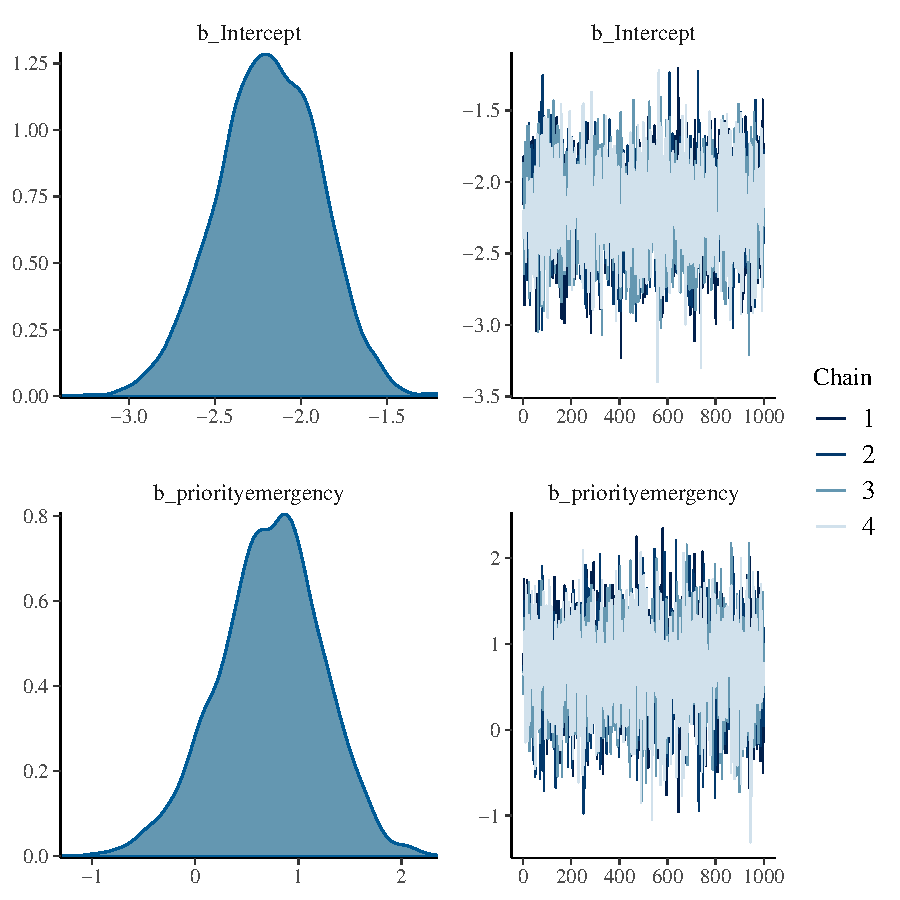
\includegraphics[width=\maxwidth]{prop-bayesprop2-1} }

\end{Schunk}

\begin{Schunk}
\begin{Sinput}
# Bring out posterior draws
w <- as.data.frame(f)
b0 <- w[, 'b_Intercept']
b1 <- w[, 'b_priorityemergency']
r  <- rbind(c(mean(b0), median(b0), pmode(b0)),
            c(mean(b1), median(b1), pmode(b1)),
            c(mean(exp(b1)), median(exp(b1)), pmode(exp(b1))))
colnames(r) <- c('Posterior Mean', 'Posterior Median', 'Posterior Mode')
rownames(r) <- c('b0', 'b1', 'OR')
round(r, 3)
\end{Sinput}
\begin{Soutput}
   Posterior Mean Posterior Median Posterior Mode
b0         -2.188           -2.184         -2.203
b1          0.724            0.748          0.865
OR          2.333            2.113          1.721
\end{Soutput}
\end{Schunk}

Because the prior on the OR is conservative, the Bayesian posterior mode for the OR is smaller than the frequentist maximum likelihood estimate of 2.87.  

Below notice how easy it is to do Bayesian inference on derived quantities p1 and p2 which are functions of b0 and b1.

\begin{Schunk}
\begin{Sinput}
# 0.95 credible interval for log odds ratio and odds ratio
quantile(b1, c(0.025, 0.975))
\end{Sinput}
\begin{Soutput}
     2.5%     97.5% 
-0.326236  1.656346 
\end{Soutput}
\begin{Sinput}
quantile(exp(b1), c(.025, 0.975))
\end{Sinput}
\begin{Soutput}
    2.5%    97.5% 
0.721635 5.240131 
\end{Soutput}
\begin{Sinput}
exp(quantile(b1,  c(0.025, 0.975)))
\end{Sinput}
\begin{Soutput}
     2.5%     97.5% 
0.7216349 5.2401303 
\end{Soutput}
\begin{Sinput}
# Posterior density of emergency:other odds ratio
plot(density(exp(b1)), xlab='OR', main='')
abline(v=c(1, pmode(exp(b1))), col=gray(0.85))
# Probability that OR > 1
P(exp(b1) > 1)
\end{Sinput}
\begin{Soutput}
[1] 0.91875
\end{Soutput}
\begin{Sinput}
# Probability it is > 1.5
P(exp(b1) > 1.5)
\end{Sinput}
\begin{Soutput}
[1] 0.74925
\end{Soutput}
\begin{Sinput}
# Probability that risk with emergency surgery exceeds that of
# non-emergency (same as P(OR > 1))
# plogis in R is 1/(1 + exp(-x))
P(plogis(b0 + b1) > plogis(b0))
\end{Sinput}
\begin{Soutput}
[1] 0.91875
\end{Soutput}
\begin{Sinput}
# Prob. that risk with emergency surgery elevated by more than 0.03
P(plogis(b0 + b1) > plogis(b0) + 0.03)
\end{Sinput}
\begin{Soutput}
[1] 0.8165
\end{Soutput}


\centerline{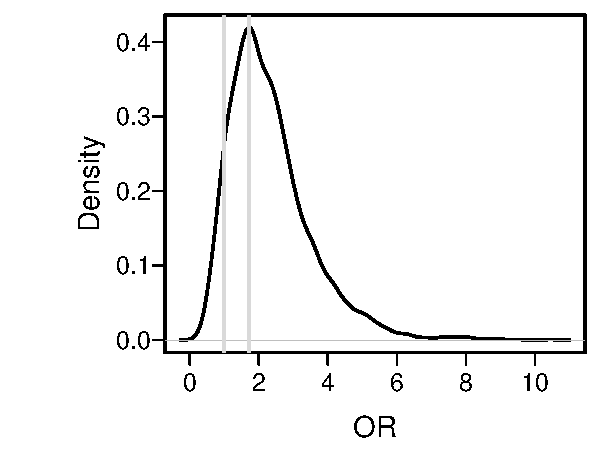
\includegraphics[width=\maxwidth]{prop-bayesprop4-1} }

\end{Schunk}

Even though the priors for the intercept and log odds ratio are independent, the connection of these two parameters in the data likelihood makes the posteriors dependent as shown with Spearman correlations of the posterior draws below.  Also get the correlation between evidence for the two probabilities.  These have correlated priors even though they are unconnected in the likelihood function.  Posteriors for $p_1$ and $p_2$ are less correlated than their priors.

\begin{Schunk}
\begin{Sinput}
cor(b0, b1, method='spearman')
\end{Sinput}
\begin{Soutput}
[1] -0.4439781
\end{Soutput}
\begin{Sinput}
cor(plogis(b0), plogis(b0 + b1), method='spearman')
\end{Sinput}
\begin{Soutput}
[1] 0.1385611
\end{Soutput}
\end{Schunk}


To demonstrate the effect of a skeptical prior:
\bi
\item Add random grouping to model as we did with the frequentist analysis
\item Make use of prior information that this variable is unlikely to be important
\item Put a prior on the log OR for this variable centered at zero with chance that the OR $> 1.25$ of only 0.05
\ei

\begin{Schunk}
\begin{Sinput}
normsolve(0, log(1.25), 0.05)
\end{Sinput}
\begin{Soutput}
[1] 0.1356616
\end{Soutput}
\begin{Sinput}
p <- c(prior(normal(-2.944, 1.216), class='Intercept'),
       prior(normal(0, 0.857),      class='b', coef='priorityemergency'),
       prior(normal(0, 0.136),      class='b', coef='random'))

f2 <- brm(death ~ priority + random, data=d, prior=p, family='bernoulli',
          seed=121, refresh=FALSE)
\end{Sinput}
\begin{Sinput}
f2
\end{Sinput}
\begin{Soutput}
 Family: bernoulli 
  Links: mu = logit 
Formula: death ~ priority + random 
   Data: d (Number of observations: 136) 
Samples: 4 chains, each with iter = 2000; warmup = 1000; thin = 1;
         total post-warmup samples = 4000

Population-Level Effects: 
                  Estimate Est.Error l-95% CI u-95% CI Rhat Bulk_ESS Tail_ESS
Intercept            -2.16      0.31    -2.82    -1.61 1.00     2804     2922
priorityemergency     0.71      0.50    -0.27     1.66 1.00     3614     3020
random               -0.06      0.13    -0.31     0.19 1.00     3879     3110

Samples were drawn using sampling(NUTS). For each parameter, Eff.Sample 
is a crude measure of effective sample size, and Rhat is the potential 
scale reduction factor on split chains (at convergence, Rhat = 1).
\end{Soutput}
\end{Schunk}

\bi
\item Effect of \co{random} is greatly discounted
\item Posterior mean priority effect and its credible interval is virtually the same as the model that excluded \co{random}
\ei

James Rae and Nils Reimer have written a nice tutorial on using the \R~\co{brms} package for binary logistic regression available at
\href{http://bit.ly/brms-lrm}{bit.ly/brms-lrm}
